\documentclass[9pt]{report}

\usepackage{talks}

\begin{document}

\sf%
\mbox{ }
\\[12pt]
\spc{{\LARGE\bfseries \color{MidnightBlue}{Solving Inverse Problems}}}
\\[4pt]
\spc{\LARGE\bfseries \color{MidnightBlue}{with Bayesian Inference}}
\\[36pt]
\noindent 
\spc{\large\bfseries \color{MidnightBlue}{Bob Carpenter}}
\\[2pt]
\spc{\small Center for Computational Mathematics}
\\[2pt]
\spc{\small Flatiron Institute}
\vfill 
\noindent 
\spc{\footnotesize March 2024}
\hfill 
{\footnotesize \url{https://mc-stan.org}}
\hfill 

\includegraphics[width=0.3in]{img/new-logo.png}

\sld{Uncertainty}
\begin{itemize}
\item permeates \myemph{science} and \myemph{
    decision making}
\item in the form of
\begin{subitemize}
\item \myemph{sampling} uncertainty,
\item \myemph{measurement} uncertainty, and
\item \myemph{modeling} uncertainty.
\end{subitemize}
\vfill
\item The \myemph{alternative to good statistics} is
\begin{subitemize}
\item not no statistics,
\item but \myemph{bad statistics}. \hfill (Bill James)
\end{subitemize}
\end{itemize}

\sld{Probability \& Statistics}
\begin{itemize}
\item Probability theory uses math to \myemph{quantify uncertainty}.
\item \myemph{Bayesian statistics} applies probability theory to
\begin{subitemize}
\item data {analysis},
\item {prediction} \& forecasting,
\item model {evaluation}, and
\item {decision} theory.
\end{subitemize}
\item The \myemph{computational bottlenecks} are
\begin{subitemize}
\item model expression and
\item posterior inference.
\end{subitemize}
\end{itemize}


% \sld{Probability is \textit{\bfseries not} $\ldots$}
% {\linespread{1.3}
% \small\linespread{1.35}
% \begin{quote}\linespread{1.5}An intellect which at a certain
%   moment would know all forces that set nature in motion, and all
%   positions of all items of which nature is composed, if this
%   intellect were also vast enough to submit these data to analysis, it
%   would embrace in a single formula the movements of the greatest
%   bodies of the universe and those of the tiniest atom; \myemph{for such an
%   intellect nothing would be uncertain} and the future just like the
%   past would be present before its eyes.
%   \vfill\linespread{1.25}
%   -- \footnotesize \myemph{Pierre-Simon Laplace}. 1814.  \textit{A
%     Philosophical Essay on Probabilities}.  Translated by
%   F.~W.~Truscott and F.~L.~Emory, 1951.  
% \end{quote}
% }


\sld{Probability is $\ldots$}
{\linespread{1.3}
\small
\begin{quote}
\myemph{Every event is
in itself certain, not probable}; if we knew all, we should either know
positively that it will happen, or positively that it will not. But
its \myemph{probability} to us means the \myemph{degree of expectation of its
occurrence, which we are warranted in entertaining by our present
evidence}.
\vfill\linespread{1.25}
-- \footnotesize \myemph{John Stuart Mill}.  1882.  \textit{A System
  of Logic: Ratiocinative and Inductive}. Eighth edition.  III:18.
\end{quote}
}

\sld{The chance of rain in Edinburgh?}
\begin{itemize}
\item What's the chance of rain in Edinburgh, Scotland?
\begin{subitemize}
\item if it could be any day of the year: 52\%
\item if I know the month is October: 55\%
\item if I also know it's 24h from now: 55\%
\item if I also have today's weather report: 80\%
\item if it's now and I see rain: 100\%
\end{subitemize}
\item The world didn't change, our knowledge of it did.
  \vfill
\item Coin flips are the same!
\end{itemize}


\sld{Simulate some Baseball (clinical trials)}
%
\begin{itemize}
\item True .300 on base percentage (OBP) then simulate
\begin{subitemize}
\item {\bfseries 10 at bats} \hfill (.000 to .600 OBP)
\\[4pt] 1 1 2 6 2 0 4 4 4 2
\vspace*{3pt}
%
\item {\bfseries 100 at bats} \hfill (0.220 to 0.330 OBP)
\\[4pt] 22 34 30 26 25 31 31 28 27 33
\vspace*{3pt}
%
\item {\bfseries 1000 at bats} \hfill (.294 to .320 OBP)
\\[4pt] 296 307 302 298 290 297 303 294 280 320
\vspace*{3pt}
%
\item {\bfseries 10,000 at bats} \hfill (.295 to .305 OBP)
\\[4pt] 3022 2953 2987 2946 2994 2989 3052 3024 3038 2938
\end{subitemize}
\end{itemize}




\mypart{}{Bayesian Inference}

\sld{Notation}
\begin{itemize}
\item Variables
\begin{subitemize}
\item $y$ : \myemph{data} (observed)
\item $\theta$ : \myemph{parameters} (unknown)
\end{subitemize}
\item Probability functions
\begin{subitemize}
\item $p(y, \theta)$ : \myemph{joint} density
\item $p(y \mid \theta)$ : \myemph{sampling} density
{\footnotesize \hfill (\myemph{likelihood} as fun of $\theta$)}
\item $p(\theta)$ : \myemph{prior} (parameter marginal)
\item $p(\theta \mid y)$ : \myemph{posterior}
\item $p(y)$ : \myemph{evidence} (data marginal)
\end{subitemize}
\end{itemize}

\sld{Bayes's rule}
{\footnotesize
\begin{eqnarray*}
p(\theta \mid y) & = & \frac{p(y, \theta)}{p(y)}
\\[4pt]
& = & \frac{p(y \mid \theta) \cdot p(\theta)}{p(y)}
\\[4pt]
& = & \frac{p(y \mid \theta) \cdot p(\theta)}{\int_{\Theta} p(y, \theta) \, \textrm{d}\theta}
\\[4pt]
& = & \frac{p(y \mid \theta) \cdot p(\theta)}{\int_{\Theta} p(y \mid \theta) \cdot p(\theta) \, \textrm{d}\theta}
\\[10pt]
& \propto &
p(y \mid \theta) \cdot p(\theta).
\end{eqnarray*}
\begin{subitemize}
\item \myemph{Posterior} proportional to \myemph{likelihood times prior}
\end{subitemize}
}

\sld{Estimates, events, and predictions}
\begin{itemize}
\item \myemph{Parameter estimate}
$$
\hat{\theta}
\ = \ \mathbb{E}\!\left[\theta \mid y\right]
\ = \
\int_{\Theta} \theta \cdot p(\theta \mid y) \, \textrm{d}\theta
$$
\item \myemph{Event probability} ($A \subseteq \Theta$, \ \ {\footnotesize e.g., $A = \{ \theta : \theta > 0\}$})
$$
\textrm{Pr}[A \mid y]
\ = \ \mathbb{E}\!\left[\textrm{I}_A(\theta) \mid y\right]
\ = \
\int_{\Theta} \textrm{I}_A(\theta) \cdot p(\theta \mid y)
\, \textrm{d}\theta
$$
\item \myemph{Predictive inference}
$$
p(\tilde{y} \mid y)
\ = \ \mathbb{E}\!\left[p(\tilde{y} \mid \theta) \ \middle| \ y\right]
\ = \
\int_{\Theta} p(\tilde{y} \mid \theta) \cdot p(\theta \mid y)
\, \textrm{d} \theta
$$
\end{itemize}

\sld{(Markov chain) Monte Carlo}
\begin{subitemize}
\item Given \myemph{sample} $\theta^{(1)}, \ldots, \theta^{(M)} \sim p(\theta \mid y).$
\item General \myemph{plug-in expectation} calculations,
\begin{eqnarray*}
\mathbb{E}[f(\theta) \mid y]
& = &
\int_{\Theta} \, f(\theta) \cdot p(\theta \mid y) \, \textrm{d}\theta
\\[8pt]
& = &
\lim_{M \rightarrow \infty} \,
\frac{1}{M} \, \sum_{m=1}^M \, f\!\left(\theta^{(m)}\right)
\\[8pt]
& \approx &
\frac{1}{M} \, \sum_{m=1}^M \, f\!\left(\theta^{(m)}\right).
\end{eqnarray*}
\item (MCMC) central limit theorem \myemph{approx. error} $\mbox{ } \propto \frac{\displaystyle 1}{\displaystyle \sqrt{M_{(\textrm{eff})}}}$
\end{subitemize}



% \mypart{Decision Theory}

% \sld{Expected utility and risk}
% \begin{itemize}
% \item Agent has choice of \myemph{actions} $a \in A$.
% \begin{subitemize}
% \item discrete: do I go to college?
% \item continuous: how much do I invest for retirement?
% \end{subitemize}
% \item \myemph{Utility}: $\textrm{util}(a, \theta)$ based on state of world $\theta$
% \begin{subitemize}
% \item risk aversion, etc. rolled into utility
% \end{subitemize}
% \item \myemph{Expected Utility} conditioned on $y$:
% $$
% \mathbb{E}\!\left[\textrm{util}(a, \theta) \mid y\right]
% \ = \
% \int_{\Theta} \textrm{util}(a, \theta) \cdot p(\theta \mid y) \ \textrm{d}\theta.
% $$
% \item point estimates aren't plug \& play due to \myemph{non-linearity}
% \end{itemize}

% \sld{Optimal Decisions}
% \begin{itemize}
% \item Given observed data $y$ and model $p(y, \theta)$, choose action $a^* \in A$ that \myemph{maximizes expected utility}
% $$
% a^* = \textrm{arg max}_\theta \ \mathbb{E}\!\left[\textrm{util}(a, \theta) \mid y\right].
% $$
% \item \myemph{Compute} expectation via MCMC sample
% $$
% \theta^{(1)}, \ldots, \theta^{(m)} \sim p(\theta \mid y),
% $$
% as
% $$
% \mathbb{E}\!\left[\textrm{util}(a, \theta) \mid y\right]
% \ \approx \
% \frac{1}{M} \sum_{m=1}^M \textrm{util}\!\left(a, \theta^{(m)}\right)
% $$
% \item can be \myemph{automatically differentiated}.
% \end{itemize}

% \sld{Online A/B/... testing}
% \begin{itemize}
% \item discrete choice of action $k \in 1:K$ 
% \item probabilistic outcome of action $k$ as $p(y \mid \theta_k)$
% \item assume utility $\textrm{util}(\theta, a)$
% \item observe history of actions $a_1, \ldots, a_t \in 1:K$ and paired
%   outcomes $y_1, \ldots, y_t \in \mathbb{R}.$
% \item explore/exploit: 
% next action $a_{t+1}$ chosen w.\ probability proportional to $k$ being
% best (Thompson sampling)
% \vfill {\footnotesize e.g., COVID-19 and antibody testing risk reduction.}
% \end{itemize}



\mypart{Example 1}{Birth Ratio}

\sld{Birth ratio \hfill {\Large (Laplace, 1781)}}
\begin{itemize}
\item \myemph{Live births} in Paris, 1745--1770
\begin{subitemize}
\item $y = 251,527$ male, $N = 493,472$ total
\end{subitemize}
\item \myemph{Sampling}:
$p(y \mid N, \theta)
 = \textrm{binomial}(y \mid N, \theta).$
\item \myemph{Prior}:
$p(\theta)
 = \textrm{uniform}(\theta \mid 0, 1)$
\item \myemph{Posterior}:
$p(\theta \mid y)
 = \textrm{beta}(\theta \mid 1 + y, \ 1 + N - y).$
\vfill
\item {$\textrm{Pr}[\theta \in (0.508, 0.512)] = 0.99$}
\hfill {\small (estimated \myemph{male birth rate})}
\item {$\textrm{Pr}[\theta > 0.5] \approx 1 - 10^{-42}$}
\hfill {\small (``morally certain'' \myemph{more boys})}
\end{itemize}

\sld{Coding in Stan}
\begin{stancode}
data {
  int y;  // boys = 251527
  int N;  // total = 493472
}
parameters {
  real<lower=0, upper=1> theta;
}
model {
  y ~ binomial(N, theta);
  theta ~ uniform(0, 1);
}
generated quantities {
  int<lower=0, upper=1> theta_gt_half = (theta > 0.5);
  int<lower = 0> y_sim = binomial_rng(100, theta);
}
\end{stancode}

\sld{Executing}
%
\begin{codein}
> fit <- stan("laplace.stan")
> print(fit, probs=c(0.005, 0.995), digits=3)
\end{codein}
\begin{codeout}
                     mean se_mean   0.5%   99.5%
theta               0.510   0.000  0.508   0.512
theta_gt_half       1.000     NaN  1.000   1.000
y_sim              50.902   0.081 38.000  64.000
\end{codeout}
%
\begin{subitemize}
\item \myemph{estimate} $\hat{\theta}$ is posterior sample \myemph{mean} for $\theta$;
\item 99\% \myemph{interval} for $\theta$ estimated by sample \myemph{quantiles}
\item $\textrm{Pr}[\theta > 0.5]$ estimated by sample \myemph{mean of indicator}
\item {\texttt y\_sim} estimated \myemph{forecast} for next 100 births
\end{subitemize}


\mypart{}{Workflow}

\sld{Bayesian Workflow}
\begin{enumerate}
\item Design experiment \& \myemph{collect data} (its own workflow)
\item Model evaluation
\begin{subitemize}
\item \myemph{prior predictive checks}: is the prior sensible?
\item \myemph{simulation-based calibration}: does the algorithm work
  on data simulated from the model?
\item \myemph{posterior predictive checks}: does model capture
  relevant aspects of real data?
\item \myemph{hold out/cross-validation}: does model predict well?
\end{subitemize}
\item If model is lacking, \myemph{improve model and repeat (2)}
  \begin{subitemize}
  \item and if data is lacking, collect more and repeat (1)
  \end{subitemize}
\end{enumerate}

\mypart{}{Calibration}

\sld{Calibration}
\begin{itemize}
\item Empirical (frequentist) evaluation of \myemph{probabilistic forecasts}
\item Of the days on which a 75\% of rain is forecast, roughly 75\% of them
should be rainy. 
\begin{subitemize}
\item for $N$ \myemph{calibrated predictions} of probability $\theta$,
\\
$Y \sim \textrm{binomial}(N, \theta)$ will obtain
\end{subitemize}
\item Calibrated predictions for \myemph{rain in Edinburgh}:
\begin{subitemize}
\item 52\% is calibrated if evaluated over random days of the year.
\item Prediction based on average for day of month is calibrated
  (i.e., 65\% for December)
\item Is {\small \url{weather.com}}'s forecast calibrated?  Empirical question.
\end{subitemize}
\end{itemize}

\sld{Sharpness}
\begin{itemize}
\item Sharp probabilistic predictions have \myemph{low entropy}.
\item \myemph{Narrowly concentrated} predictions are sharper
\begin{subitemize}
\item $\mbox{Pr}[\alpha \in (.58, .59)] = .9$ sharper than
$\mbox{Pr}[\alpha \in (.5, .6)] = .9$
\end{subitemize}
\item Probabilistic predictions \myemph{nearer 0 or 1} are sharper
\begin{subitemize}
\item $\mbox{Pr}[z_i = 1] = 0.95$ sharper than $\mbox{Pr}[z_i = 1] = 0.6$
\end{subitemize}
\end{itemize}

\sld{Inference evaluation criterion}
\begin{itemize}
\item For probabilistic forecasts:
\begin{center}
  \myemph{Maximize sharpness subject to calibration.}
\end{center}
\item \myemph{Goal}: consistent, useful inference from \myemph{finite data}.
\begin{subitemize}
\item cf. minimize variance subject to zero bias for estimators
\end{subitemize}
\item Bayesian models are calibrated if they are \myemph{well-specified}
\begin{subitemize}
\item i.e., they capture the true data-generating process.
\item But, models are always approximate.
\item So, need to test fit to real data and predictions.
\end{subitemize}
\end{itemize}



\mypart{Example 2}{Population Dynamics}

\sld{Population Dynamics \hfill {\large (Volterra 1926)}}
\begin{itemize}
\item populations at time $t$ of prey $u(t)$ \& predator $v(t)$
\item Volterra's mechanistic model
$$
\frac{\textrm{d}}{\textrm{d}t}u = (\alpha - \beta \cdot v) \cdot u
\qquad
\frac{\textrm{d}}{\textrm{d}t}v = (-\gamma + \delta \cdot u) \cdot v
$$
\vspace*{-12pt}
\begin{subitemize}
\item $\alpha$: prey growth rate;  \ $\beta$: predation shrinkage
\item $\gamma$: predator shrinkage; \ $\delta$: predation growth
\end{subitemize}
\end{itemize}

\sld{Analytic solution \hfill {\large (Volterra 1926)}}
\begin{center}
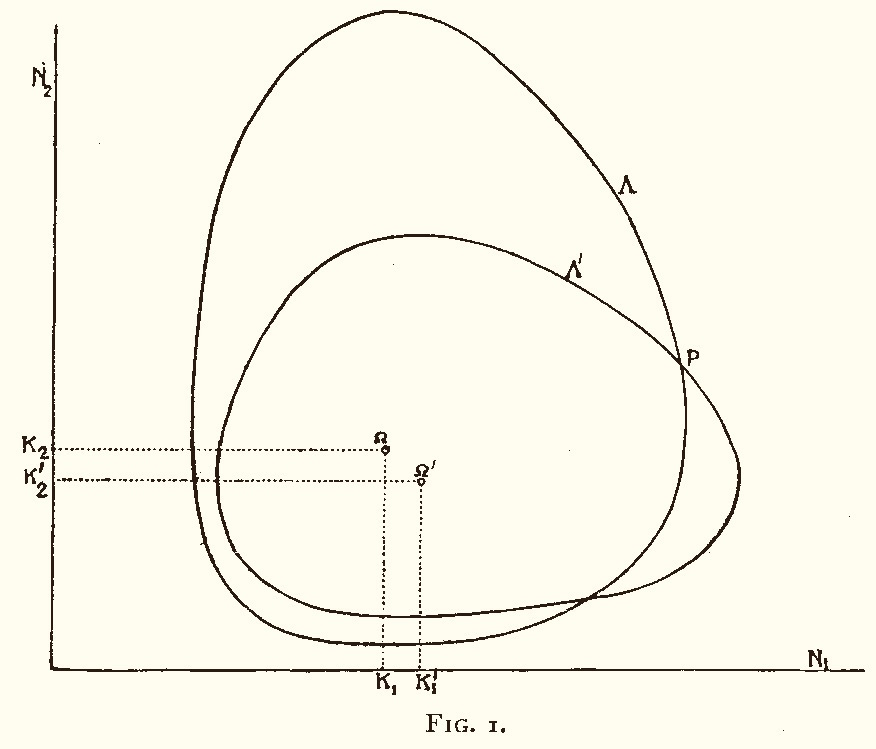
\includegraphics[width=0.6\textwidth]{img/volterra-solutions.jpg}
\end{center}

\sld{Knowns and Unknowns}

\begin{itemize}
\item \myemph{Knowns}
  \begin{subitemize}
  \item number of pelts collected at each time
  \end{subitemize}
\item \myemph{Unknowns}
  \begin{subitemize}
  \item initial populations
  \item subsequent populations
  \item growth and shrinkiage parameters $\alpha, \beta, \gamma, \delta$
  \end{subitemize}
\end{itemize}

\sld{Measurement/model error}
\begin{itemize}
\item $u, v$ are observed
\item $\hat{u}, \hat{v}$ predicted by mechanistic model
\item Independent \myemph{error proportional to population} size
\begin{subitemize}
\item $u_t \sim \textrm{lognormal}(\hat{u}_t, \sigma_1)$
\item $v_t \sim \textrm{lognormal}(\hat{v}_t, \sigma_2)$
\end{subitemize}
\item Weakly informative \myemph{priors determine scale}
\begin{subitemize}
\item $\alpha, \gamma \sim \textrm{normal}(1, 0.5)$; \ \ \
$\beta, \delta \sim \textrm{normal}(0.05, 0.05)$
\item $\sigma_1, \sigma_2 \sim \textrm{lognormal}(-1, 1)$
\end{subitemize}
\end{itemize}

\sld{Assumptions}
\begin{itemize}
\item pelts are a reasonable proxy for the populations 
  \begin{subitemize}
  \item could try to validate with mark/recapture 
  \end{subitemize} 
\item population only depends on population of predator and prey 
  \begin{subitemize}
  \item no outside shocks like weather, epidemics, other predators, etc. 
  \end{subitemize}
\item rough scale of solutions known ahead of time 
\item measurement error is proportional to population size 
\end{itemize}


\sld{Normal and log normal}
\begin{itemize}
\item Normal density is the usual bell curve, with
  \[
    \textrm{normal}(y \mid \mu, \sigma) \propto \frac{1}{\sigma} \exp\left(-\frac{1}{2}
      \left( \frac{y - \mu}{\sigma} \right)^2\right)
  \]
\item If $y$ has a $\textrm{normal}(\mu, \sigma)$ distribution, then
  $\exp(y)$ has a $\textrm{lognormal}(\mu, \sigma)$ distribution.
\item 95\% intervals for normal are roughly $\mu \pm 2\sigma$
\item 95\% intervals for lognormal are roughly
  \[
    \exp(\mu \pm 2\sigma) = \exp(\mu) 
  {\footnotesize \begin{array}{c} \times \\[-4pt]
    \div \end{array}} \exp(2\sigma)
  \]
\end{itemize}

\sld{The Lynx and the Hare}

\begin{itemize}
  \item \myemph{Lynx} (left) are predators who prey almost exclusively on
    \myemph{snowshoe hares} (right) 
\end{itemize}
\begin{center}
  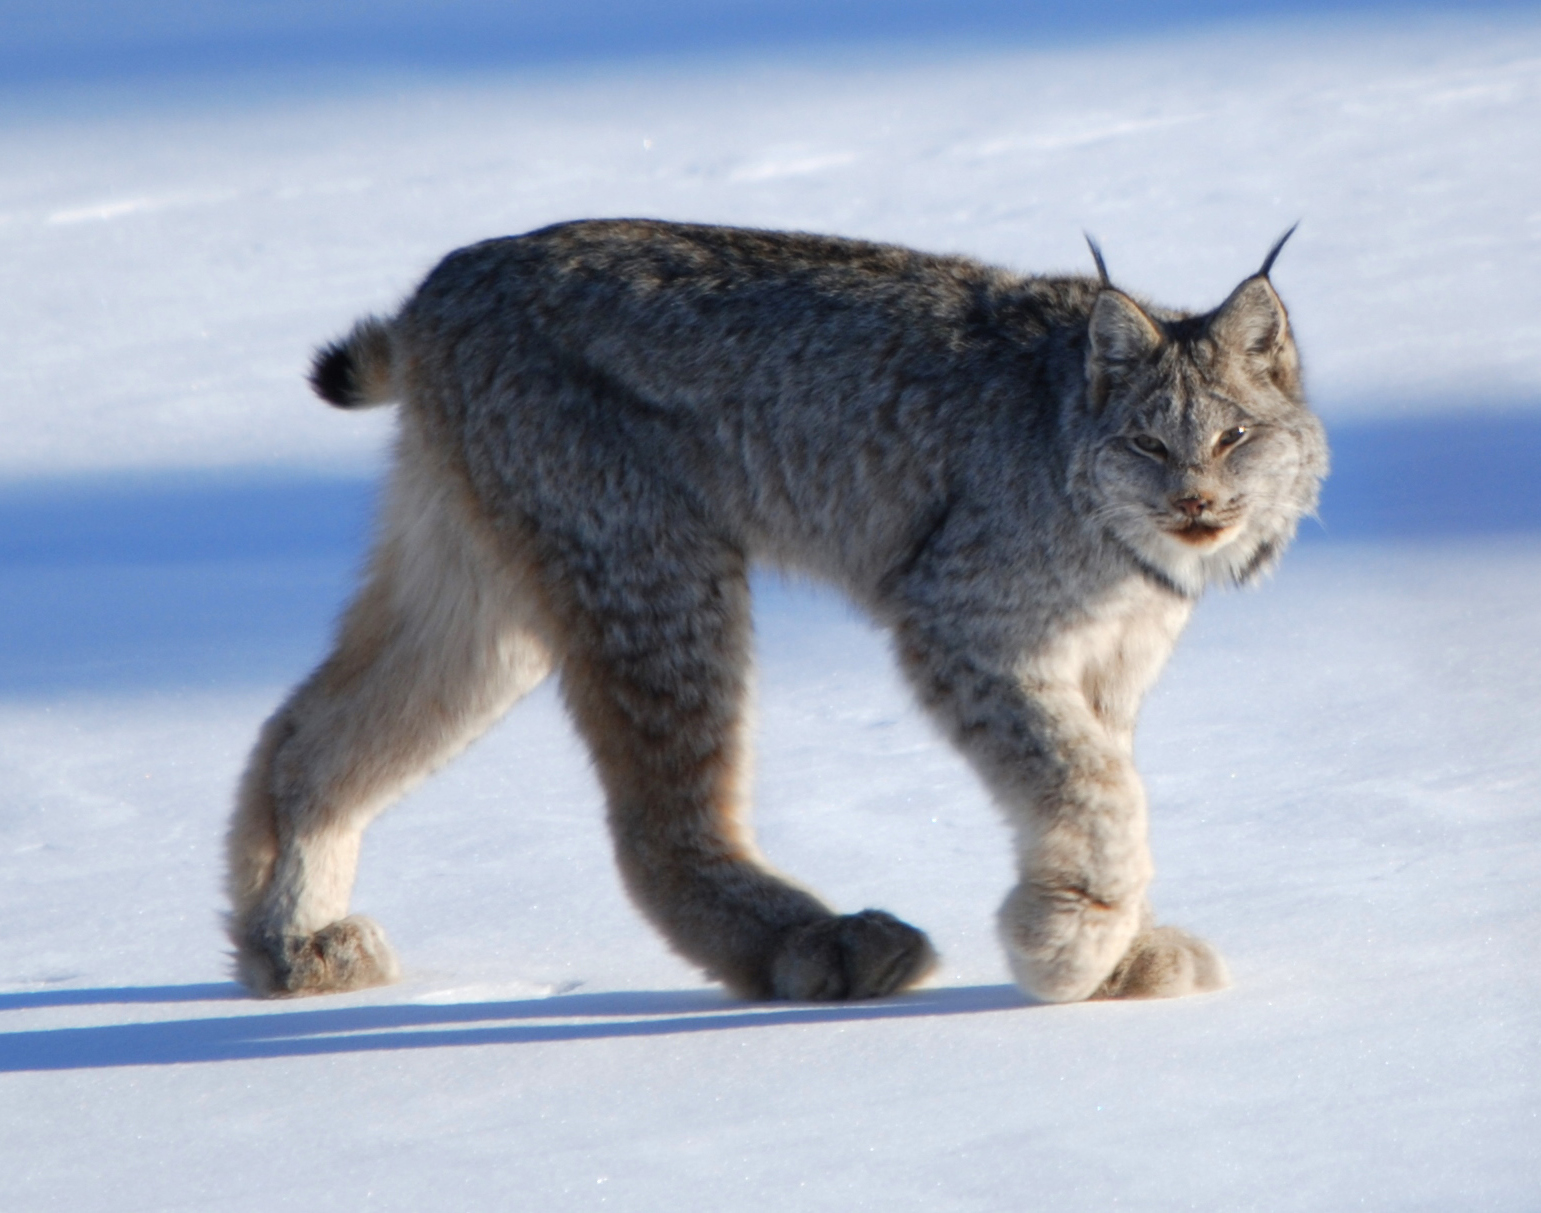
\includegraphics[height=0.35\textwidth]{img/lynx.jpeg}
  \quad
  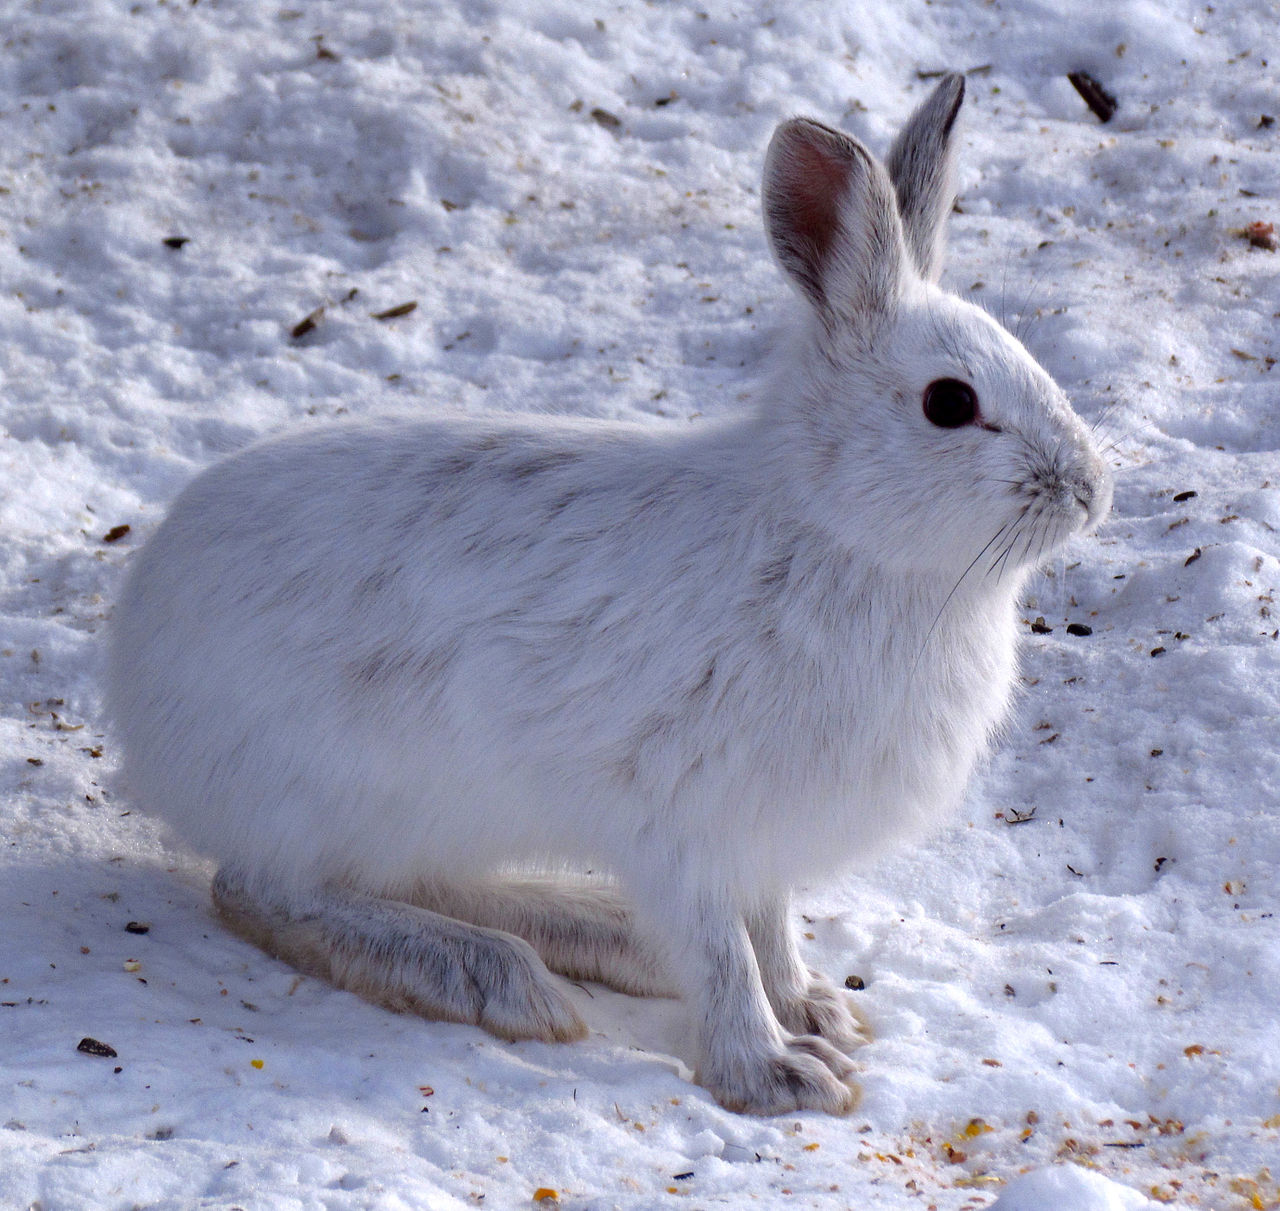
\includegraphics[height=0.35\textwidth]{img/hare.jpeg}
\end{center}
\begin{itemize}
  \item But it's very labor intensive to count animals with standard
    mark/recapture techniques
\end{itemize}

\sld{Hudson's Bay Co.\ pelts \hfill {\large (Hewitt 1921)}}
\begin{itemize}
  \item A proxy is the number of animals captured for pelts.
\end{itemize}
\begin{center}
  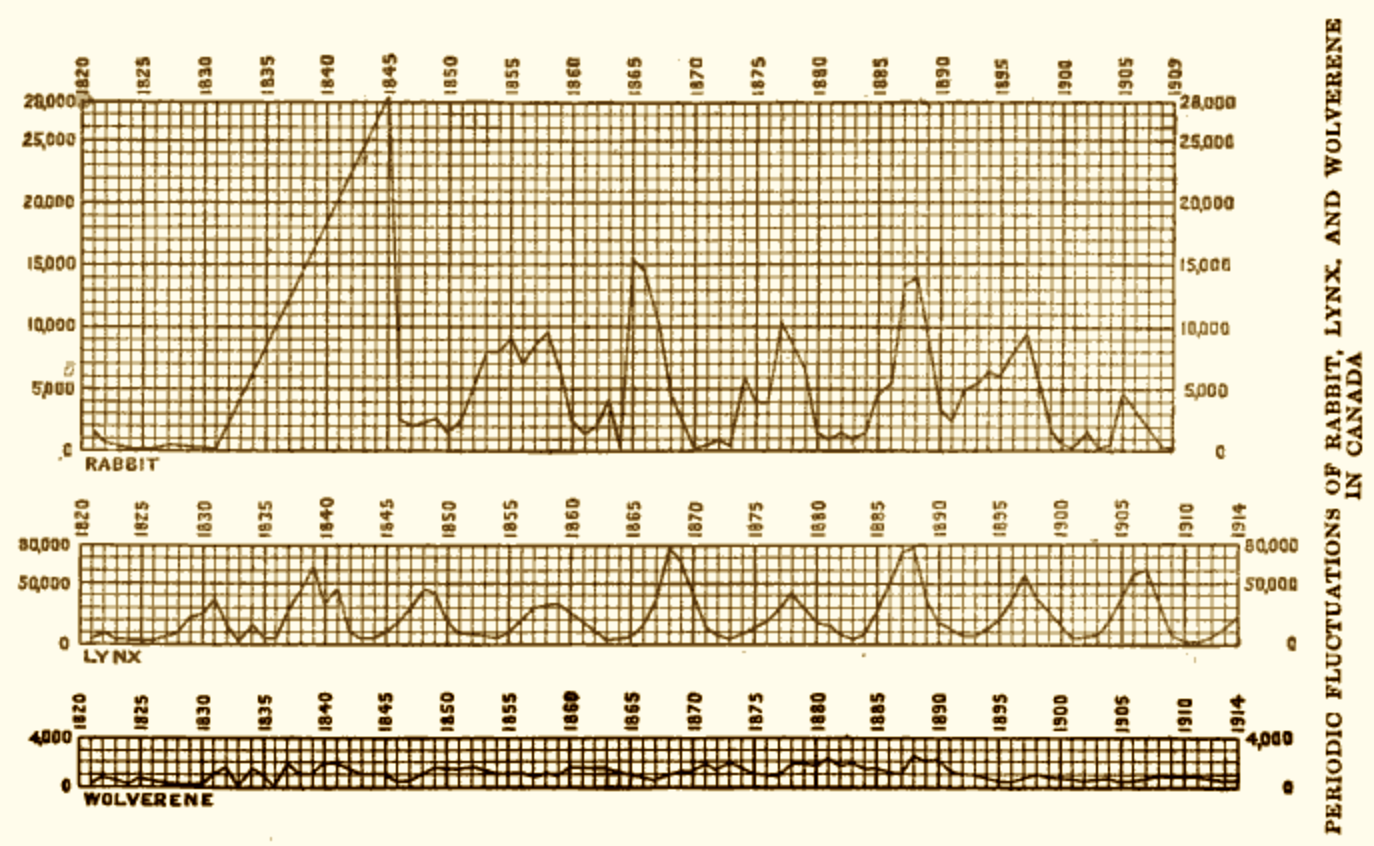
\includegraphics[width=0.8\textwidth]{img/hudons-bay-data.png}
\end{center}

\sld{Plotted pelt data}
\begin{center}
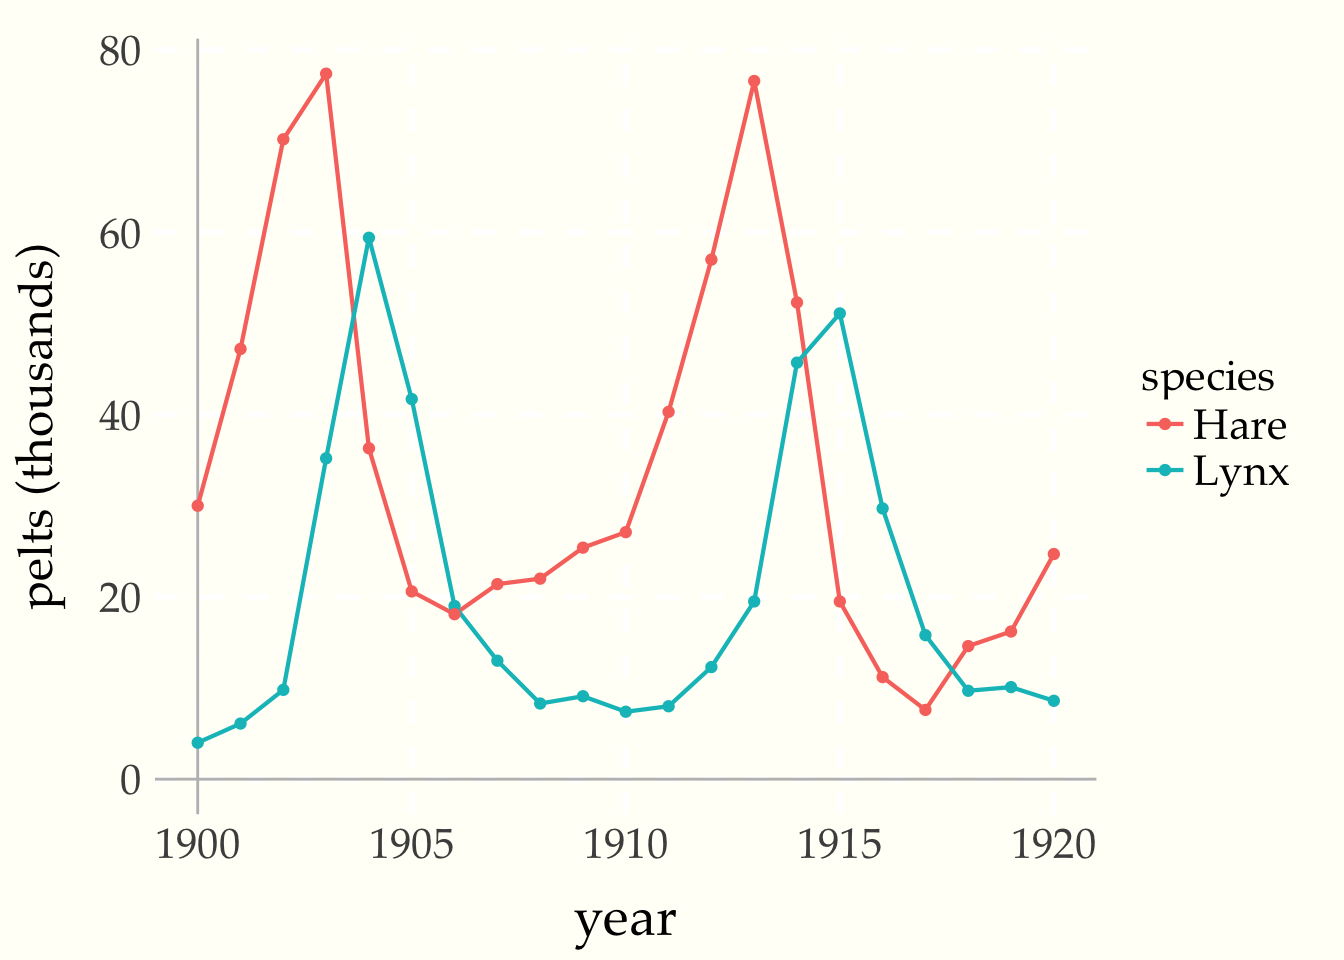
\includegraphics[width=0.45\textwidth]{img/lynx-hares-1.png}~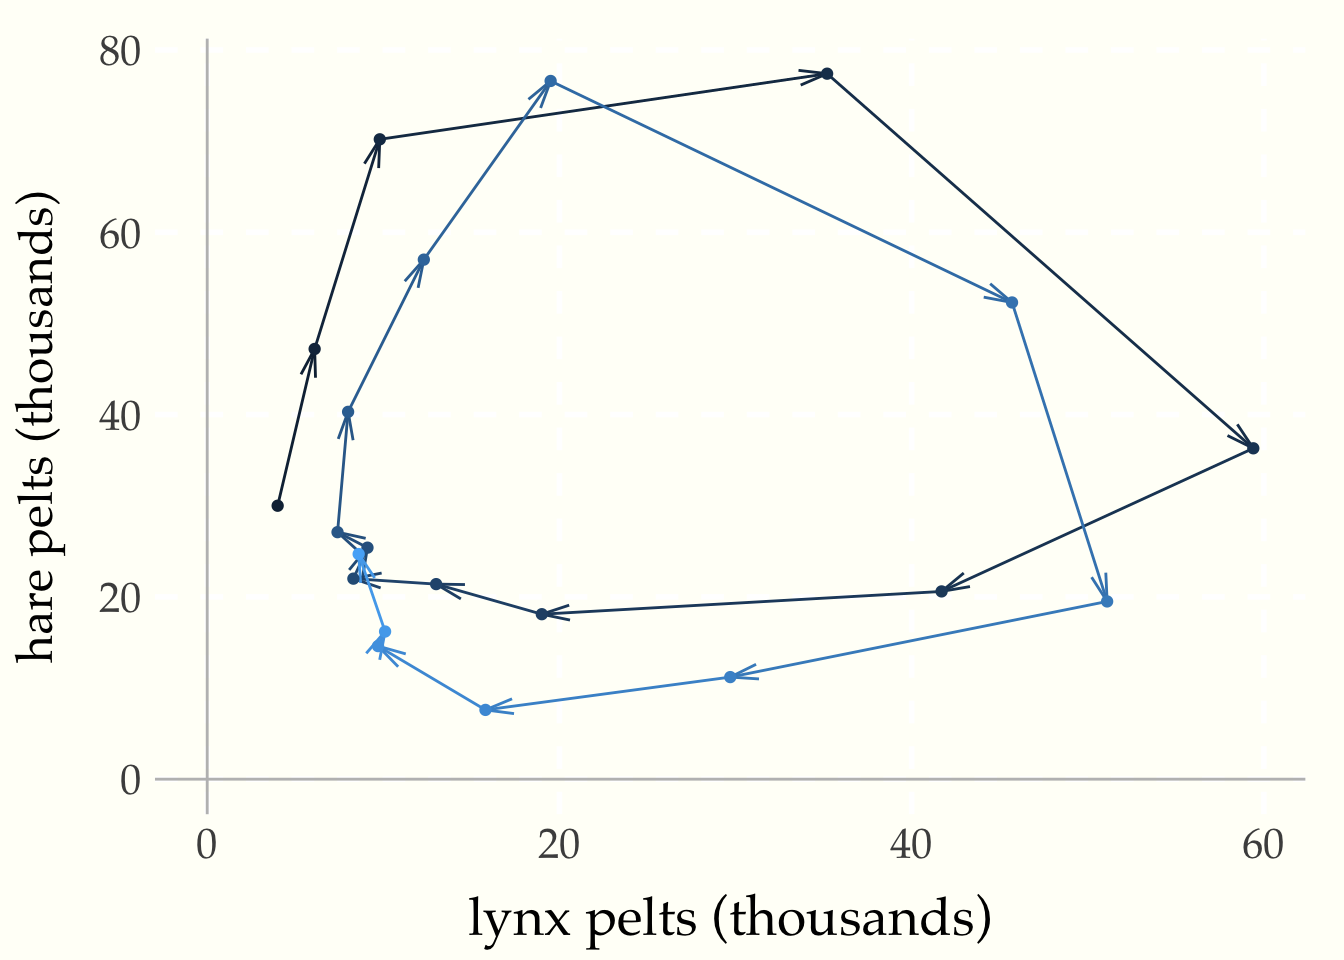
\includegraphics[width=0.45\textwidth]{img/lynx-hares-2.png}
\end{center}
\begin{itemize}
\item {\it left)} pelts vs. time \hfill
{\it right)} hare vs. lynx pelts
\\
(line per species) \hfill (over time)
\item pelt data assumed proportional to population
\item w/o modeling relation, \myemph{model predicts pelts}
\end{itemize}

\sld{Stan dynamics \& error}
\begin{stancode}
real[] duv_dt(real t, real[] uv, real[] theta,
              real[] theta, real[] x_r, int[] x_i) {
  return { (theta[1] - theta[2] * uv[2]) * uv[1],
           (-theta[3] + theta[4] * uv[1]) * uv[2] };
}
...
real uv_hat[T, 2]
  = integrate_ode(duv_dt, z0, t0, sol_ts[1:T], theta,
                  rep_array(0.0, 0), rep_array(0, 0));
...
y[1:T, 1] ~ lognormal(uv_hat[1:T, 1], sigma_u);  // prey
y[1:T, 2] ~ lognormal(uv_hat[1:T, 2], sigma_v);  // predator
\end{stancode}

\sld{Measurements \& predictions}
\begin{subitemize}
\item measured pelts (red) vs.\ fitted model and predictions (blue)
\end{subitemize}
\begin{center}
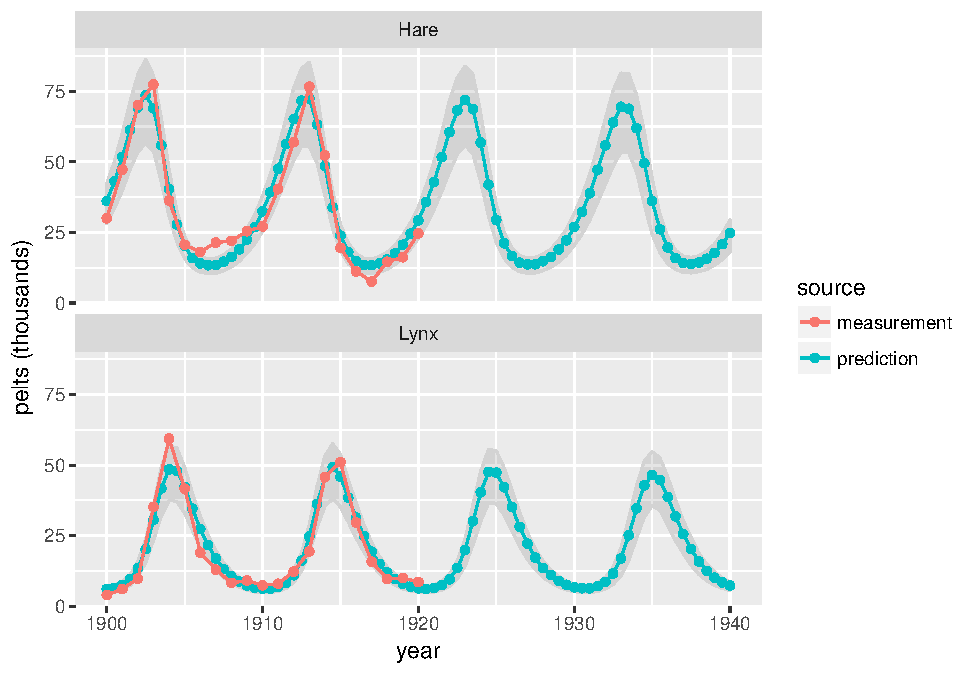
\includegraphics[width=0.7\textwidth]{img/lotka-volterra-posterior.pdf}
\end{center}

\sld{100 predictive draws}
\begin{center}
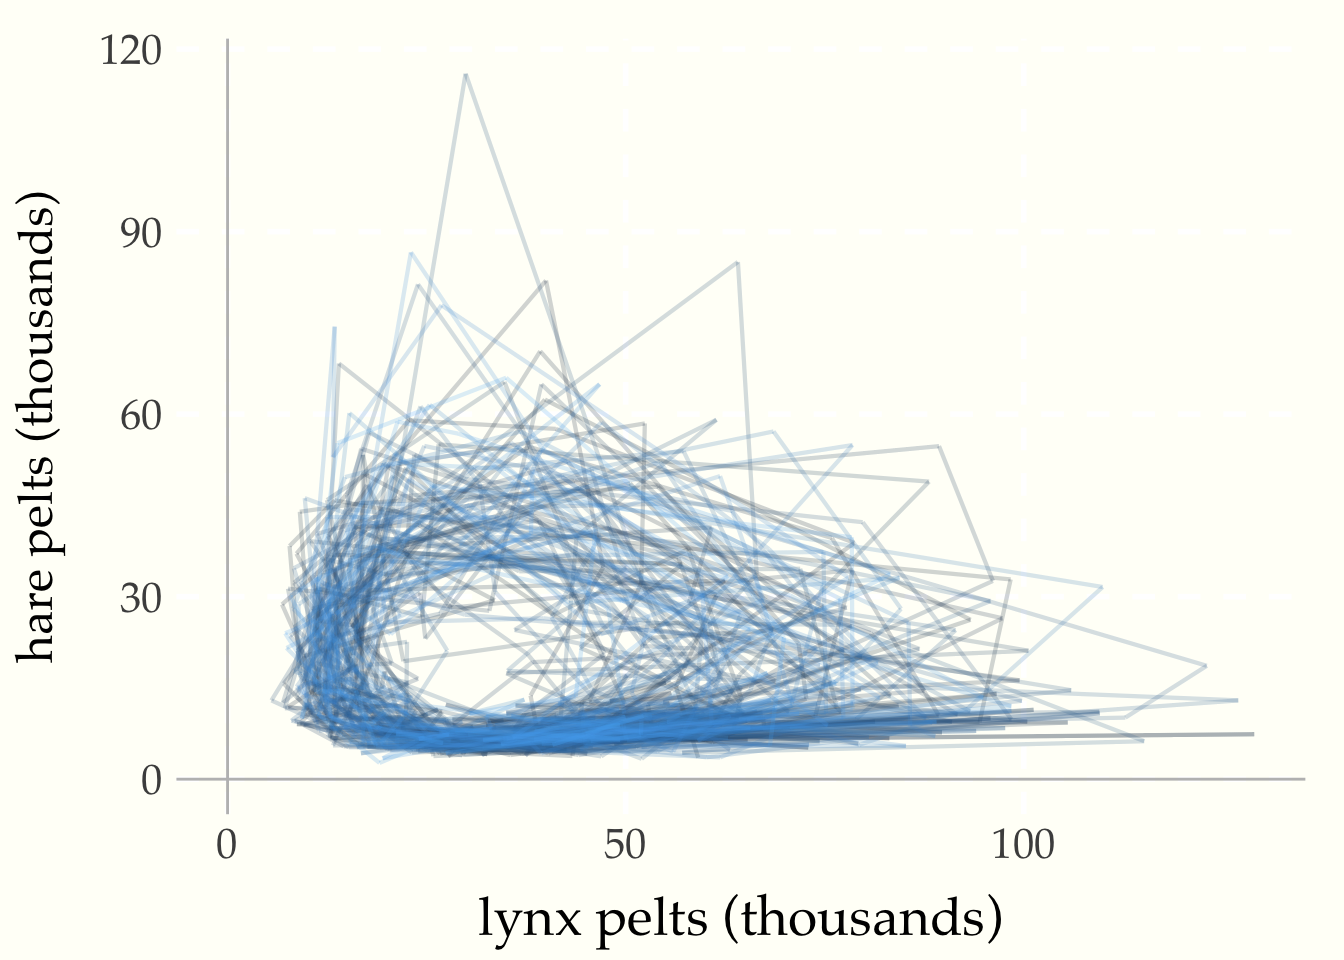
\includegraphics[width=0.8\textwidth]{img/lotka-volterra-posterior-time.png}
\end{center}

\sld{Identification of parameters?}

\begin{itemize}
\item Posterior mean estimates minimize expected square error,
  \[
    \hat{\alpha} = \mathbb{E}[\alpha \mid y]
    = \textrm{arg min}_{\alpha'} \ \mathbb{E}[(\alpha' - \alpha)^2 \mid
    y].
  \]
\item Given the Hudson's Bay data, the estimates are
  \[
    \hat{\alpha} = 0.55
    \quad
    \hat{\beta} = 0.028
    \quad
    \hat{\gamma} = 0.80
    \quad
    \hat{\delta} = 0.024
  \]
%  \item The error scales are identical (multiplicative, related)
  \[
    \hat{\sigma}_1 = 0.25 \qquad \hat{\sigma}_2 = 0.25
  \]
  \item Posterior intervals are quite wide
    \begin{subitemize}
    \item $\textrm{Pr}[0.45 \leq \alpha \leq 0.63] = 0.8 \quad \textrm{Pr}[0.023 \leq \beta \leq 0.033] = 0.8$
    \item $\textrm{Pr}[0.69 \leq \gamma \leq 0.91] = 0.8 \quad 
      \textrm{Pr}[0.020 \leq \delta \leq 0.029] = 0.8$
    \item $\textrm{Pr}[0.20 \leq \sigma_1 \leq 0.31] = 0.8 \quad 
      \textrm{Pr}[0.20 \leq \sigma_2 \leq 0.31] = 0.8$
    \end{subitemize}
  \end{itemize}

\sld{Summary}
\begin{itemize}
\item mechanistic forward model of dynamics (Lotka 1926)
\begin{subitemize}
\item $\hat{y} = f(\theta)$
\end{subitemize}
\item error model $y_{t,k} \sim \textrm{lognormal}(\hat{y}_{t,k}, \sigma_k)$
\item added weakly informative priors $p(\theta)$ (fixing scale) 
\item Stan turns the Bayesian crank to sample from posterior
\begin{subitemize}
\item $\theta^{(1)}, \ldots, \theta^{(M)} \sim p(\theta \mid y).$
\end{subitemize}
\item Estimates are sample means; intervals are sample quantiles;
  predictions are plug-in estimates
\item This methodology \myemph{works for many scientific models}.
\end{itemize}


\mypart{}{AI, ML, and Statistics}

\sld{What is Artificial Intelligence (AI)?}
\begin{itemize}
\item AI is about pushing frontier of ``thinking'' computers
  \begin{subitemize}
  \item playing Go, driving a car, translating natural language,
    recognizing images, $\ldots$
  \end{subitemize}
\item AI is not about a technique
  \begin{subitemize}
  \item according to Google and the European Union, regression is AI!
  \end{subitemize}
\item machine learning (ML) is more difficult to characterize
\end{itemize}

\sld{Machine Learning (ML) and Stats (1)}
\begin{itemize}
\item Traditional stats focuses on data analysis
\item Traditional ML focuses on prediction
  \begin{subitemize}
  \item this is why ML is eating stats' lunch
  \end{subitemize}
\item Bayesian stats is about data analysis \textsl{and} prediction
\end{itemize}
 
\sld{ML and Stats (2)}
\begin{itemize}
\item Models
  \begin{subitemize}
  \item Stats focuses on interpretable, tractable parametric models
  \item ML focuses on black-box, intractable, non-parametric models
  \end{subitemize}
\item Inference
  \begin{subitemize}
  \item ML focuses on prediction based on plug-in point estimates
  \item traditional stats focuses on estimates, confidence intervals,
    and hypothesis tests
  \item Bayesian stats focuses on calibrated posterior uncertainty
    and uses probability for everything
  \end{subitemize}
\end{itemize}

\sld{ML and Stats (3)}
\begin{itemize}
\item Scale
  \begin{subitemize}
  \item ML focuses largely on ``big'' data
  \item Stats tries to squeeze info out of small data
  \item Stats can build more model with more data (spatio-temporal,
    sub-population, etc.)
  \item ML models tend to be more flexible and also scale with data
  \end{subitemize}
\end{itemize}

\mypart{}{Questions / Comments?}

\mypart{}{Stan}

\sld{What is Stan?}
%
\begin{itemize}
\item a domain-specific \myemph{probabilistic programming language}
\item Stan \myemph{program} defines a \myemph{differentiable} probability model
  \begin{subitemize}
  \item declares data and (constrained) parameter variables
  \item defines log posterior (or penalized likelihood)
  \item defines predictive quantities
  \end{subitemize}
\item Stan \myemph{inference} fits model \& makes predictions
  \begin{subitemize}
  \item MCMC for full Bayesian inference
  \item variational and Laplace for approximate Bayes
  \end{subitemize}
\item \footnotesize Carpenter, B., Gelman, A., Hoffman, M. D., Lee, D., Goodrich, B., Betancourt, M., Marcus Brubaker, Jiqiang Guo, Peter Li, Riddell, A. (2017). Stan: A probabilistic programming language. {\slshape J.\ Stat.\ Soft.} 76(1).
\end{itemize}



\sld{Availability \& Usage}
\begin{subitemize}
\item \textit{Platforms:} \ Linux, Mac OS X, Windows
\vspace*{-4pt}
\item \textit{Interfaces:} \ R, Python, Julia, MATLAB, Mathematica
\vspace*{-4pt}
\item \textit{Developers (academia \& industry):} 40+ \ {\small (15+ FTEs)}
\vspace*{-4pt}
\item \textit{Users:}\ tens or hundreds of thousands
\vspace*{-4pt}
\item \textit{Companies using:} \ hundreds or thousands
\vspace*{-4pt}
\item \textit{Downloads:}\ millions
\vspace*{-4pt}
\item \textit{User's Group:} \ 3000+ registered; 6000+ non-bot views/day
\vspace*{-4pt}
\item \textit{Books using:} \ 10+
\vspace*{-4pt}
\item \textit{Courses using:} \ 100+
\vspace*{-4pt}
\item \textit{Case studies about:} 100+
\vspace*{-4pt}
\item \textit{Articles using:} \ 3000+
\vspace*{-4pt}
\item \textit{Conferences:} 4 (800+ attendance)
\end{subitemize}

\sld{Some published applications}
%
\begin{subitemize}
\item \myemph{Physical sciences}: {\footnotesize
astrophysics, statistical mechanics, particle physics, (organic) chemistry, geology, oceanography, climatology, biogeochemistry, materials science, $\ldots$
}
\vspace*{-3pt}
\item \myemph{Biological sciences}: {\footnotesize
molecular biology, clinical drug trials, entomology, pharmacology,
toxicology, opthalmology, neurology, genomics, agriculture, botany, fisheries,
epidemiology, population ecology, neurology, psychiatry, $\ldots$
}
\vspace*{-3pt}
\item \myemph{Social sciences}: {\footnotesize
 econometrics (macro and micro), population dynamics, cognitive
 science, psycholinguistics, social networks, political science,
 survey sampling, anthropology, sociology, social work, $\ldots$
}
\vspace*{-3pt}
\item \myemph{Other}: {\footnotesize education, public health, A/B testing,
government, finance, machine learning, logistics, electrical engineering,  transportation, actuarial science, sports, advertising, marketing, $\ldots$}
\end{subitemize}

\sld{Industries using Stan}
\vspace*{3pt}
\begin{subitemize}
\item \myemph{marketing attribution}: Google, Domino's Pizza, Legendary Ent.
\item \myemph{demand forecasting}: Facebook, Salesforce
\item \myemph{financial modeling}: Two Sigma, Point72
\item \myemph{pharmacology \& CTs}: Novartis, Pfizer, Astra Zeneca
\item \myemph{(e-)sports analytics}: Tampa Bay Rays, NBA, Sony Playstation
\item \myemph{survey sampling}: YouGov, Catalist
\item \myemph{agronomy}: Climate Corp., CiBO Analytics
\item \myemph{real estate pricing models}: Reaktor
\item \myemph{industrial process control}: Fero Labs
\end{subitemize}


\sld{Why is Stan so Popular?}
\vspace*{3pt}
\begin{subitemize}
\item \myemph{Community}: large, friendly, helpful, and sharing
\item \myemph{Documentation}:  novice to expert; breadth of fields
\item \myemph{Robustness}:  industrial-strength code; user diagnostics
\item \myemph{Flexibility}:  highly expressive language;  large math lib
\item \myemph{Portability}: popular OS, language, and cloud support
\item \myemph{Extensibility}: developer friendly; derived packages
\item \myemph{Speed}:  $2-\infty$ orders of magnitude faster
\item \myemph{Scalability}:  2+ orders of magnitude more scalable
\item \myemph{Openness}: permissive code and doc licensing
\end{subitemize}


\mypart{}{What Stan Does}

\sld{No-U-turn sampler}
%
\vspace*{-3pt}
\begin{itemize}
\item \myemph{Hamiltonian Monte Carlo} (HMC)
\begin{subitemize}
\item \myemph{Potential Energy}: negative log posterior $-\log p(\theta \mid y)$
\item \myemph{Kinetic Energy}: random standard normal each iteration
\item \myemph{geometric ergodicity} for wider range of models \& data
\end{subitemize}
  %
\item Adapt leapfrog algorithm \myemph{during warmup}
  \vspace*{-4pt}
  \begin{itemize}\small
  \item step size adapted to target acceptance rate
  \item Euclidean metric estimated w.\ sample covariance
  \end{itemize}
  %
\item Adapt leapfrog algorithm  \myemph{during sampling}
  \begin{subitemize}
  \item simulate forward and backward in time until U-turn
  \item multinomial sample trajectory propto energy; bias furthest
  \end{subitemize}
  %
\item developed concurrently w. Stan (Hoffman \& Gelman 2011)
\end{itemize}

\sld{NUTS vs.\ Gibbs and Metropolis}
%
\begin{center}
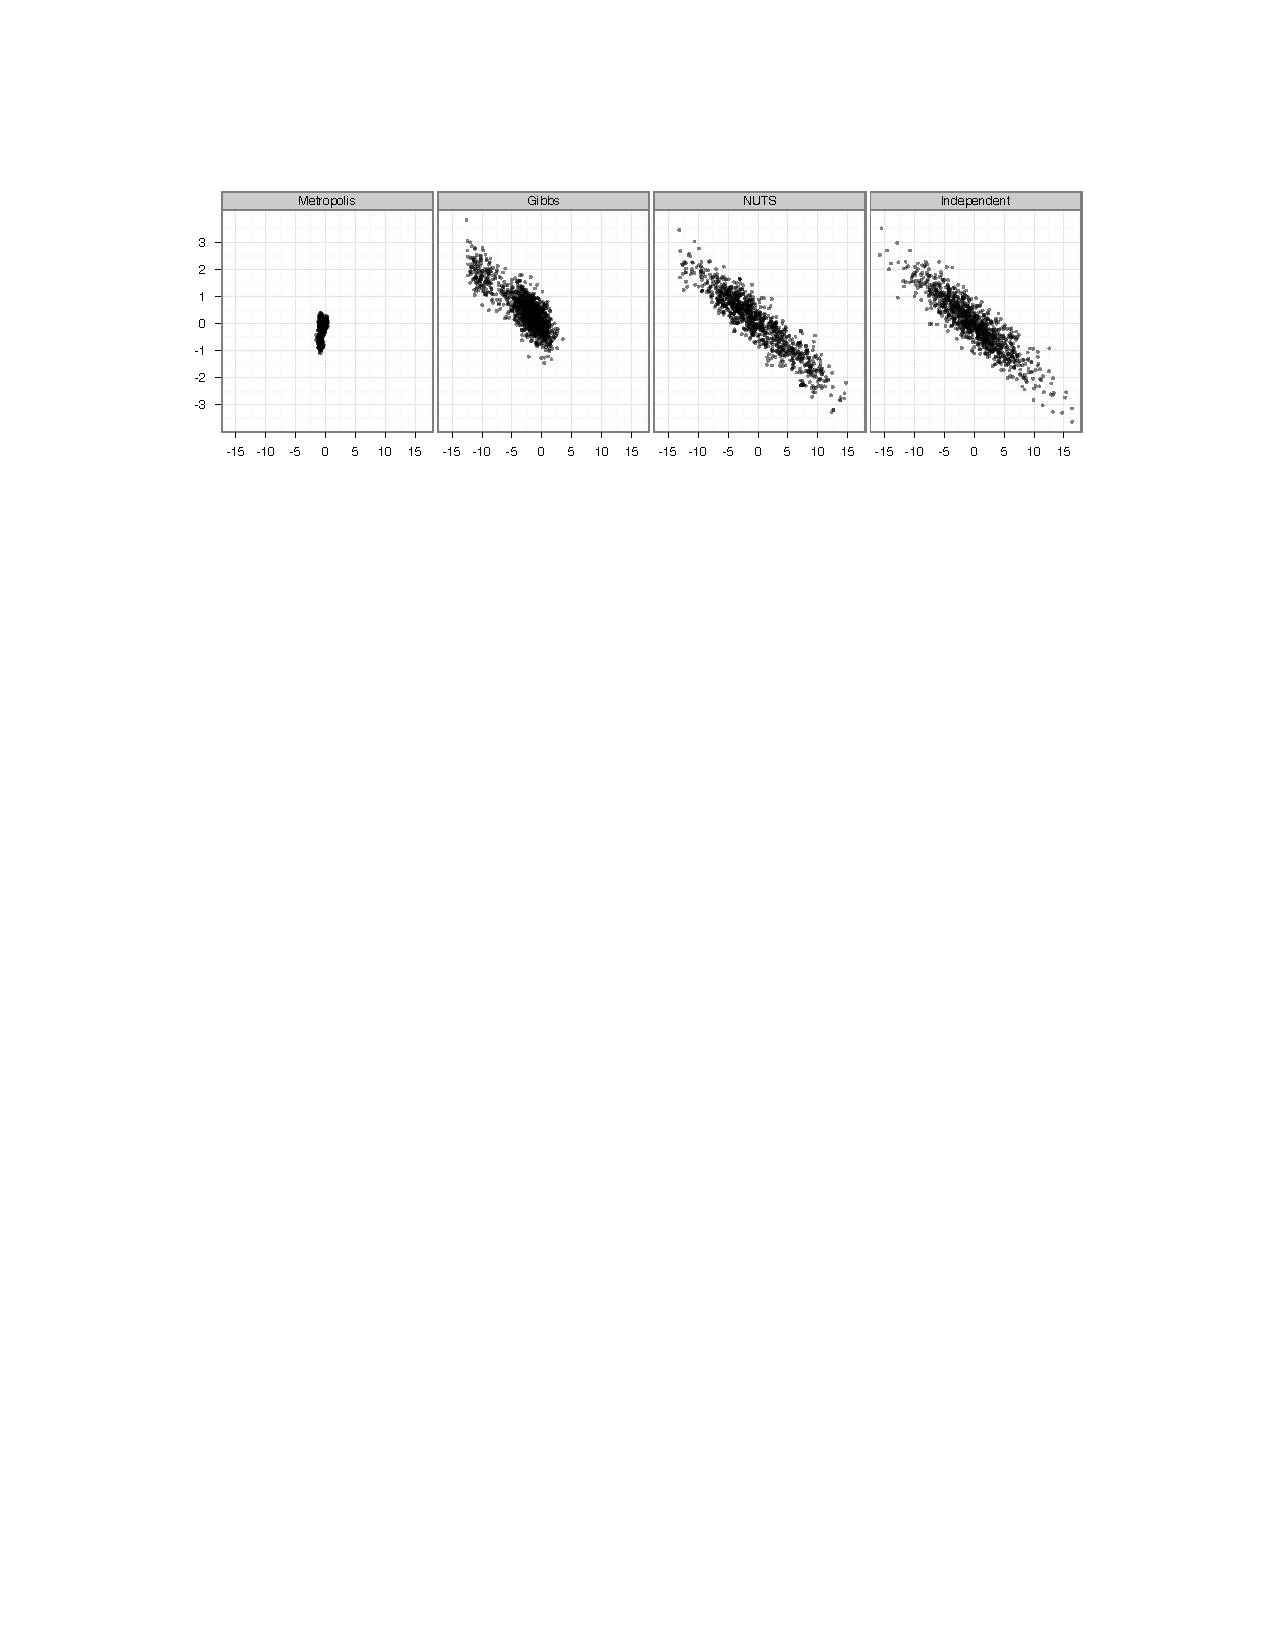
\includegraphics[width=0.9\textwidth]{img/nuts-vs.pdf}
\end{center}
\begin{subitemize}
\item Two dimensions from highly correlated 250-dim normal
\item \myemph{1,000,000 draws} from Metropolis and Gibbs (thinned to 1000)
\item \myemph{1000 draws} from NUTS; 1000 independent draws
\end{subitemize}

\sld{Reverse-mode autodiff (adjoint)}
\begin{itemize}
\item Build up expression graph with values $x$ and adjoints $\overline{x}$
\item Differentiating $f:\mathbb{R}^N \rightarrow \mathbb{R}$ is additional $\mathcal{O}(1)$
\item Set final result $y$'s adjoint $\overline{y} = 1$ and proceed in reverse
\item Example:  scalar $c = \log a$
\begin{subitemize}
\item $\overline{a} \ {+}{=} \ \overline{c} \cdot \frac{\displaystyle 1}{\displaystyle a}$
\end{subitemize}
\item Example: scalar $c = a \cdot b$
\begin{subitemize}
\item $\overline{a} \ {+}{=} \ \overline{c} \cdot b$; \ \ \ \ \
$\overline{b} \ {+}{=} \ \overline{c} \cdot a$
\end{subitemize}
\item Example: matrix $C = A^{-1}$
\begin{subitemize}
\item $\overline{A} \ {+}{=} \ -C^{\top} \cdot \overline{C} \cdot C^{\top}$
\end{subitemize}
\end{itemize}

\sld{Stan's Autodiff vs.\ Alternatives}
%
\vspace*{-4pt}
\begin{itemize}
\item Stan is \myemph{fastest} (and uses least memory)
\begin{subitemize}
\item among open-source C++ alternatives
\end{subitemize}
\end{itemize}
\vspace*{-8pt}
\mbox{ } \hfill \hfill
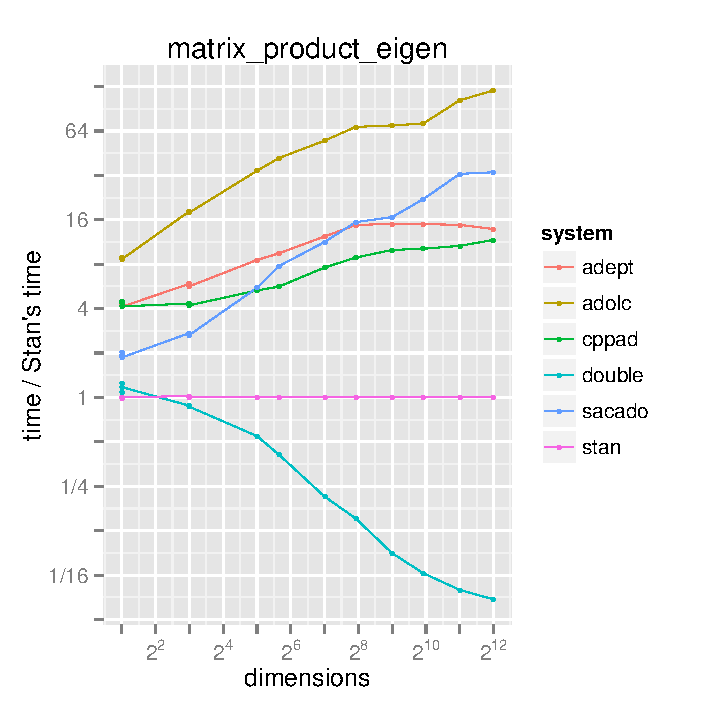
\includegraphics[width=0.40\textwidth]{img/autodiff-eval-matrix-product-eigen.pdf}
\hfill
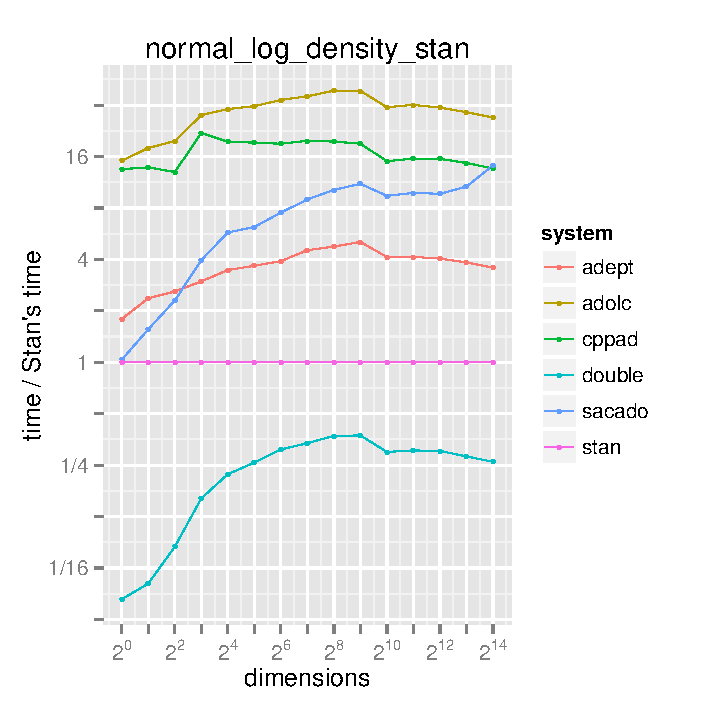
\includegraphics[width=0.40\textwidth]{img/autodiff-eval-normal-density.pdf}
\begin{subitemize}
\item \footnotesize Carpenter, B. et al. (2015). The Stan math library: Reverse-mode automatic differentiation in C++. {\slshape arXiv:}1509.07164
\end{subitemize}

\sld{Forward-mode autodiff (tangent)}
\begin{itemize}
\item Build tangents forward with values $x$ and tangents $\dot{x}$
\item Differentiating $f:\mathbb{R} \rightarrow \mathbb{R}^M$ is additional $\mathcal{O}(1)$
\item To differentiate w.r.t.\ $x$, set $\dot{x} = 1$ and work forward
\item Example:  scalar $c = \log a$
\begin{subitemize}
\item $\dot{c} = \dot{a} \cdot \frac{\displaystyle 1}{\displaystyle a}$
\end{subitemize}
\item Example: scalar $c = a \cdot b$
\begin{subitemize}
\item $\dot{c} = \dot{a} \cdot b + \dot{b} \cdot a$
\end{subitemize}
\item Example: matrix $C = A^{-1}$
\begin{subitemize}
\item $\dot{C} = -C \cdot \dot{A} \cdot C$
\end{subitemize}
\end{itemize}

\sld{Higher-order autodiff}
\begin{itemize}
\item Open up new algorithms exploiting curvature
\begin{subitemize}
\footnotesize
\item Riemannian HMC, nested Laplace approximations (ala INLA),
nested Jacobians for ODE solver, Newton solvers for optimizers and nested algebraic equations
\end{subitemize}
\item Considering log densities $f :\mathbb{R}^N \rightarrow \mathbb{R}$
\item Second-order derivatives
\begin{subitemize}
\item nest reverse in forward adds $\mathcal{O}(N)$
\item nest forward in forward $\mathcal{O}(N^2)$
\end{subitemize}
\item Third-order derivatives
\begin{subitemize}
\item nest reverse in forward in forward $\mathcal{O}(N^2)$
\item nest forward in forward in forward $\mathcal{O}(N^3)$
\end{subitemize}
\end{itemize}

\sld{Stan's shortcomings}
\begin{itemize}
\item Failures
\begin{subitemize}
\item extreme varying posterior curvature (stiff---can't adapt)
\item floating point (e.g., log cdfs and ccdfs, gradients)
\item scalability of data and parameters
\end{subitemize}
\item Missing features
\begin{subitemize}
\item black-box log densities (cf. emcee in Python)
\item checkpointed autodiff for large Gaussian processes
\item filtering (online model updating)
\item stochastic algebraic \& differential eqs, PDEs
\item structured data types, sparse data types \& closures
\end{subitemize}
\end{itemize}

\sld{Discrete parameters?}
\begin{itemize}
\item \myemph{Stan's focus}: tractably \myemph{marginalized}
\begin{subitemize}
\item e.g., mixtures, HMMs, state-space models
\item \myemph{efficient} in theory due to Rao-Blackwell; in practice by eliminating combinatorics; much better tail behavior
\item marginalizations available wherever you find EM \& MML
\end{subitemize}
\item \myemph{Out of scope}: combinatorially \myemph{intractable}
\begin{subitemize}
\item e.g., selection, clustering, random trees, neural nets
\item optimization is NP-hard or worse
\item thus \myemph{nobody knows how to get right} answer in general
\item some special cases can be fit
\end{subitemize}
\item \myemph{In between}: missing count data
\end{itemize}
 

\end{document}

